\documentclass[10pt]{jarticle}
\usepackage{float}
\usepackage{adrobo_abst}
\usepackage[dvipdfmx]{graphicx}
\usepackage{amssymb,amsmath}
\usepackage{bm}
\usepackage[superscript]{cite}
\usepackage{enumerate}
\usepackage{url}
%\usepackage[absolute]{textpos}

\renewcommand\citeform[1]{(#1)}

\begin{document}
    
    \makeatletter
    \doctype{2023年度卒業論文概要}
    \title{人のような描き方ができる頭部の線画生成の研究}{}
    \etitle{The research for the drawing robot to generate line drawings of a person's head}{}
    
    \author{20C1119\hspace{.5zw}森田大雅}
    \eauthor{Hiromasa Morita}
    
    \makeatother
    
    \abstract{In this study, we examined how to draw and made robot that draw like people. This robot starts to draw from the head on the left side. For that, we prepare a region and detect end points of edges. The reson is because in the case of right handed, it found me to start to draw from on the left side.}
    
    \keywords{Mechanical Engineering, Image Proceesing}
    
    \maketitle
    
    \supervisor{指導教員:藤江真也 教授}
    
    \section{緒\hspace{2zw}言}%===========================
	従来の描画ロボットの研究は生成された絵の結果について着目している研究が多い.
	本研究では、人のような描き方をする描き順についての研究を行う.


    \section{目的}
    
	描画ロボットの研究において、シンプルにエッジ抽出から人物画を描く文献\cite{1}や、エッジ抽出とハッチングから芸術的な人物画を鉛筆で描く文献\cite{2}、リモートユーザがタブレットを介してロボットに描かせる文献\cite{3}などが存在する.
	これらの研究では模写や芸術的な表現が可能になっているが、人のような描き方を追求したものが少ないと感じた.
	そこで本研究ではある画家が描いた頭部作品の画像から描き順ができるだけ人に近い描き方をする描画ロボットを作成する.
	頭部は表情から絵に様々な意味を連想させたり、静止した一場面にストーリーをもたらしたりする魅力がある.
	また、背景などの他の要素をより際立たさせることもできる.
    
    \section{システム構成}
	
	\subsection{Hardware}
	AdeeptのADA031を用いている.
	Arduinoで動作するため、画像処理の難易度が高い.
	そこで基盤をRaspberry\ Piに代え、それとロボットアームのservoモータに接続するためにブレッドボードやジャンパー線、抵抗を用いて改良した.
	
	\subsection{ロボットの機構}
	本研究で用いるロボットは3軸のマニピュレータロボットである.
	servo1を原点、各servoモータの関節角を$\theta_1, \theta_2, \theta_3$、各リンクの長さ$l_1, l_2, l_3, l_4$とし、逆運動学問題を解く.
	またリンク座標系を定める方法として、DH記法(Denavit-Hartenberg記法)を用いる.

    \begin{center}
        \begin{figure}[h]
            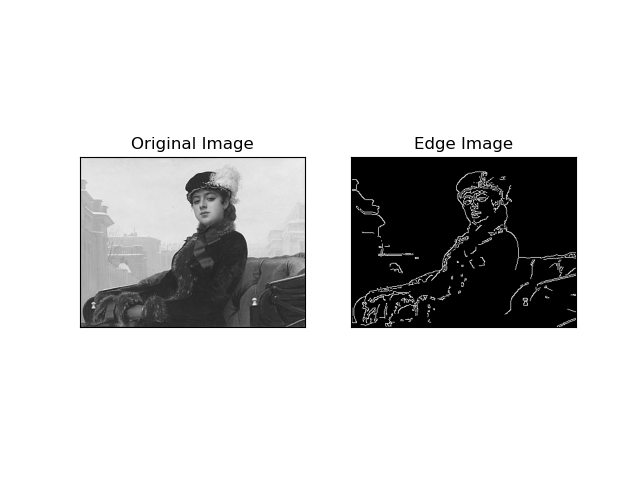
\includegraphics[width=0.5\textwidth]{/home/morita/ros2_ws/Memo/tex/img/Figure_1.png}
            \caption{リンク座標と各パラメータ(仮)}
            \label{manipulator}
        \end{figure}
    \end{center}
    
	\subsection{手先の位置と回転角の関係}
	
	運動学、逆運動学を用いてペン先の位置を各サーボモータの回転角を導出する.
	順運動学解より手先の位置が、また順運動学解より逆運動学解がそれぞれ以下のように求まる.
	
	\scriptsize
	\begin{equation}
		\begin{array}{c}
			\begin{split}
				&  x  =  C_1(l_4C_{23}  +  l_3S_{23}  +  l_2S_2)\quad \\
				&  y  =  S_1(l_4C_{23}  +  l_3S_{23}  +  l_2S_2)\quad \\
				&  z  -  l_1  =  -l_4S_{23}  +  l_3C_{23}  +  l_2C_2\quad \\
			\end{split}
		\end{array}
	\end{equation}

	\begin{equation}
		\begin{array}{c}
			\begin{split}
				\theta_1  &  =\frac{1}{2}  cos^{-1}\biggl( \frac{x^2-y^2}{x^2+y^2} \biggr) \\
				\theta_2  &  = cos^{-1}\biggl( \frac{x^2+y^2+(z-l1)^2  +  l_2^2-l_3^2-l_4^2}{2l_2\sqrt{x^2+y^2+(z-l_1)^2}} \biggr)\\
				&\qquad\qquad  +  tan^{-1}\biggl( \frac{\sqrt{x^2+y^2}}{z-l1}\biggr) \\
				\theta_3  &  =cos^{-1}\biggl( \frac{x^2+y^2+(z-l1)^2 - l_4^2-l_3^2-l_2^2}{2l_2\sqrt{l_3^2+l_4^2}}\biggr)\\
				&\qquad\qquad + tan^{-1}\biggl( \frac{-l_4}{l_3}\biggr)\\
			\end{split}
		\end{array}
	\end{equation}
	
	\normalsize

	\subsection{エッジ抽出}
	ウィリアム・ブーグローという画家の``金髪女の横顔''という絵の画像を用いる.
	理由は背景が白でシンプルであるため、画像を読み込む際にノイズが少なく綺麗にエッジ抽出を行えると考えたからである.
	この画像から線画のためにエッジを抽出する.
	線画の生成には、OpenCVのCannyのエッジ検出アルゴリズムを用いる.
	
	
	\subsection{経路の求め方}
	本研究では、領域と端点を用いて線の経路を求める.

	頭部の線画を描くパターンを調べた.
	私は顔の輪郭から始まり首や目、鼻などの細部に移って描いていく.
	これは全体から描いたほうがパーツの位置を決めやすいからだと考えられる.
	また右利きの場合、スタートは左側から描くことが多かった.
	理由はペンを右側に傾けて持つため時計周りに円を描くのが描きやすいからだと考えられる.
	半時計周りの場合、6時から12時までの区間を描くには手を少し持ち上げて描く必要があるため、寝かせたまま描ける時計周りより不安定になる.
	
	\subsection{スタート地点の決め方}

	左側から描くためにある大きさの領域を用意した.
	領域は左上の位置が横全体の$\frac{1}{8}$、縦全体の$\frac{1}{3}$に、サイズが全体の$\frac{1}{4}$になるように設定した.
	領域が頭部の左側にあるか2つの画像で確かめた.
	\\この領域を縦方向にスキャンし、最初にエッジの画素にぶつかった位置をスタート地点に決める.

    \begin{center}
        \begin{figure}[h]
            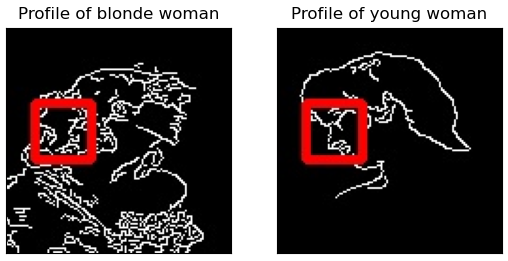
\includegraphics[width=0.45\textwidth]{/home/morita/ros2_ws/output/rectangle0709.png}
            \caption{領域の位置の確認}
            \label{the position of a region}
        \end{figure}
    \end{center}
	

	\subsection{端点の検出と線の辿り方}
	Fig.1ではエッジは綺麗に繋がって見えるが、拡大すると途切れているためロボットに座標に与えると実際の線が点線になってしまう.
	そこで端点を用いる.
	線の画素を辿り、端点まで来たら次に近くの端点に移動して描いていく.
	この処理を行うことで実際には点線を描いていくことになるが、近似的に線を描いていくような動作ができる.
  \\ 
	線の辿り方はある線の画素から隣に線の画素があるかを探し、線の画素があれば移動し、なければ最も近いまだ通過していない端点へと移動する.
	これを線の画素がなくなるまで繰り返す.
	


	\section{実験}

	経路の求めるためにラスタスキャンと領域、端点を用いた方法のどちらが人のような描き方に近いかを比較し.

    
	\section{結果}
    
	\section{結\hspace{2zw}言}%===========================
   

    \vspace{5truemm}
    {\footnotesize
        \begin{thebibliography}{99}
            
            \bibitem{1}
            M. Pichkalev, R. Lavrenov, R. Safin and K. -H. Hsia, "Face Drawing by KUKA 6 Axis Robot Manipulator," 2019 12th International Conference on Developments in eSystems Engineering (DeSE), Kazan, Russia, 2019, pp. 709-714, doi: 10.1109/DeSE.2019.00132.

			\bibitem{2}
            Felix Fisgus, Joris Wegner: ``Pankraz Piktograph'', 
            \url{https://felixfisgus.de/work/017\_pankraz\_piktograph}
            (参照日 2023年7月29日) .
            
			\bibitem{3}
            Shubham Agarwal, Sarvesh S. S. Rawat, V Sumathi: ``A drawing robotic hand based on inverse kinematics'', 
            International Conference on Information Communication and Embedded Systems (ICICES2014), Chennai, India, 2014, pp. 1-5, doi: 10.1109/ICICES.2014.7034005.

			\url{}
            (参照日 2023年7月29日) .
            
            
        \end{thebibliography}
    }
    \normalsize
    
\end{document}
